% !TeX root = ../SPL-Challenges.tex
% !TeX spellcheck = en_US
\section{Visual Referee Challenge}

\subsubsection{Challenge Goal}

In the current SPL rules, the only time that a robot is required to listen directly to the human referees is for the kick-off and goal whistle. Otherwise, all human referee decisions are communicated to the robots via electronic GameController messages. In moving towards the 2050 RoboCup goal, robots will need to directly interpret referee calls and signals (such as whistles, spoken calls and hand signals), rather than receive information from an external electronic source.

This technical challenge tests a robot's ability to identify three categories of hand signals:
\begin{enumerate}
    \item Static hand signals with one hand.
    \item Static hand signals with two hands.
    \item Dynamic (motion) hand signals with one or two hands.
\end{enumerate}

The intent of this challenge is to choose a \emph{subset} of potential referee calls in SPL games and test ability of a robot to recognize different types of hand signals in preparation for adoption in RoboCup games, rather than compile a complete set of all referee signals.

\subsubsection{Challenge setup}

One robot of the challenged team is placed in the center of the center circle facing the head referee, standing upright (stiffened) with both hands by its side. The robot should be running in the challenge mode at the start of the challenge. The team is free to choose how the software is started.

The head referee must stand on the T-junction of the center field line, opposite to the GC. The referee must wear a ``black-and-white'' striped referee jersey (if available otherwise fully black clothes) and must wear red gloves. The purpose of this clothing is to clearly distinguish the referee and their hands from background people. 

The description of this challenge and hand-signals are described based on the viewpoint of the head referee. In these descriptions from the perspective of the head referee the ``red team'' is defined as playing from left-to-right, and the ``blue team'' as playing from right-to-left. The use of colors for identifying teams is used to give equivalence to the head referee calls during SPL games \cf~\cref{fig:visual_referee_inital_positions}.

\begin{figure}[ht!]
    \begin{center}
        \leavevmode
        \includegraphics[width=1\columnwidth]{figs/referee-signals/vrc_initial.png}
        \caption{Positions of {\color{red}red}, {\color{blue}blue} team's sides, challenged robot and head referee.}
        \label{fig:visual_referee_inital_positions}
    \end{center}
\end{figure}

This challenge has \textit{five} rounds. The referee should choose 2 one-hand static signals, 2 two-hand static signals, and 1 dynamic signal. Within each type, the referee randomly chooses a hand-signal and direction. The same hand-signal may be chosen twice (with different directions). The referee should decide before the execution of the challenge starts on each runs signals and direction pair and note them down. An assistant supports the referee by showing the signal and direction, taking the timing and is also listing to the answer of the robot.

Each run works as follows:

\begin{enumerate}
    \item The referee selects a hand-signal (and direction where applicable).
    \item The referee blows the whistle once. The referee may not use one hand to hold (and blow) the whistle. The referee may instead leave the whistle held in their mouth without their hands.
    \item \qty{1}{\second} after blowing the whistle, the referee indicates the hand-signal for \qty{10}{\second}.
    \item During that time or within an additional \qty{10}{\second}, the robot must indicate the hand-signal that it has identified by:
    \begin{enumerate}
        \item Using its arm(s) to \emph{mirror} the referee's signal. That is, if the referee gives a signal for a decision for the ``red team'' using their left arm, the robot should \emph{mirror} this signal using the robot's \emph{right arm}, as the robot is facing the referee.
        \item Providing an audio phrase the referee's decision, e.g., ```Goal Red Team'''.  The exact wording is up to the team, but should clearly identify the referee's signal.
        \item The robot's gesture and voice output should be repeated until its front head button gets pressed for at least \qty{1}{\second} to indicate that the next round will start, and the robot moves back into its initial position. This should give the referee time to understand the robot's answer clearly.
    \end{enumerate}
    \item The length of time taken for the robot to indicate its interpretation from the referee blowing the whistle is measured (rounded-up to the nearest second).
    \item If the robot cannot identify the signal, it should remain motionless and provide no audio output.
    \item While not providing a hand-signal or using the whistle, the head referee must keep both hands flat and motionless by their side.
\end{enumerate}


\subsubsection{Available Hand-Signals}

Each hand-signal for the challenge is \textbf{described from the perspective of the head referee} and \textbf{pictured from the perspective of the robot}. Note that for the purpose of clarity, these do not necessarily correspond to human soccer hand-signals.

\begin{figure*}[ht!]
    \centering
    \begin{subfigure}{.33\textwidth}
        \centering
        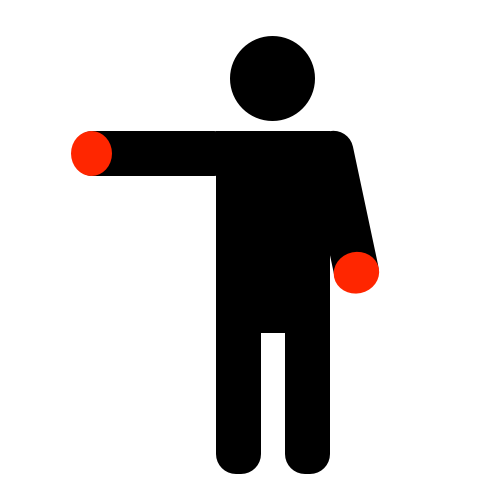
\includegraphics[height=120px]{figs/referee-signals/kick-in.png}
        \caption{\color{blue}Kick-in \textlangle{}blue\textrangle{} Team}
    \end{subfigure}
    \begin{subfigure}{.33\textwidth}
        \centering
        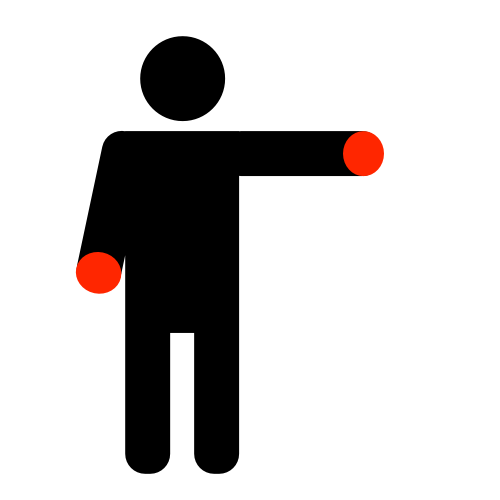
\includegraphics[height=120px]{figs/referee-signals/kick-in-flipped.png}
        \caption{\color{red}Kick-in \textlangle{}red\textrangle{} Team}
    \end{subfigure}
    \caption{\textbf{Kick-in \textlangle{}color\textrangle{} Team.} One-handed signal. One arm, extended horizontally in the direction of the half of the field corresponding to the team that receives the Kick-in Free Kick. That is, right arm extended for the ``Blue team'', and left arm extended for the ``Red team''. The non-signal hand is flat and motionless by the side of the body.}
\end{figure*}
    
\begin{figure}[ht!]
    \centering
    \begin{subfigure}{.33\textwidth}
        \centering
        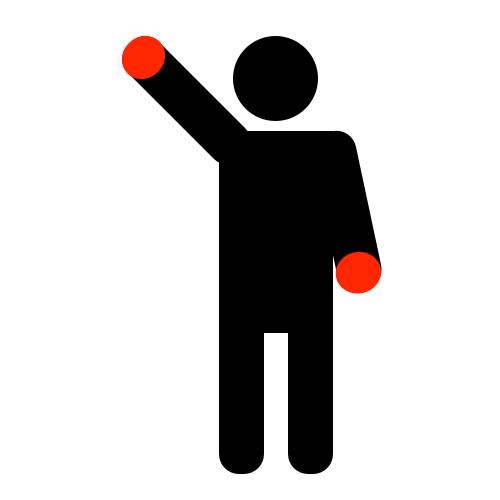
\includegraphics[height=120px]{figs/referee-signals/goal-kick.png}
        \caption{\color{blue}Goal Kick \textlangle{}blue\textrangle{} Team}
    \end{subfigure}
    \begin{subfigure}{.33\textwidth}
        \centering
        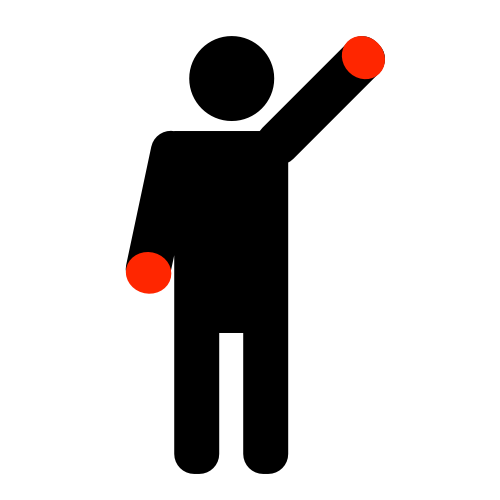
\includegraphics[height=120px]{figs/referee-signals/goal-kick-flipped.png}
        \caption{\color{red}Goal Kick \textlangle{}red\textrangle{} Team}
    \end{subfigure}
    \caption{\textbf{Goal Kick \textlangle{}color\textrangle{} Team.} One-handed signal. One arm, extended 45-degree \emph{up} in the direction of the end of the field where the goal kick will occur. That is, right arm extended for the ``Blue team'', and left arm extended for the ``Red team''. The non-signal hand is flat and motionless by the side of the body.}
\end{figure}

\begin{figure}[ht!]
    \centering
    \begin{subfigure}{.33\textwidth}
        \centering
        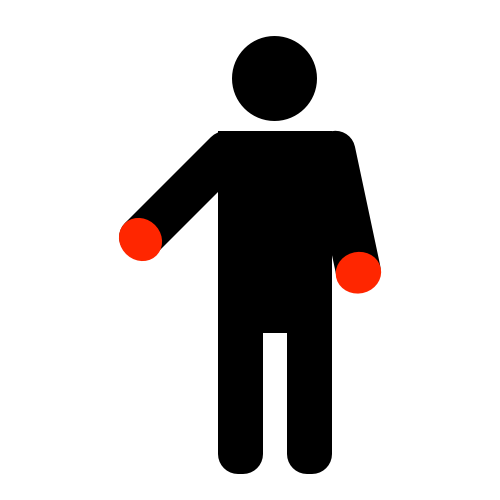
\includegraphics[height=120px]{figs/referee-signals/corner-kick.png}
        \caption{{\color{blue}Corner Kick \textlangle{}blue\textrangle{} Team}\\ (on the half of the {\color{red} red} team)}
    \end{subfigure}
    \begin{subfigure}{.33\textwidth}
        \centering
        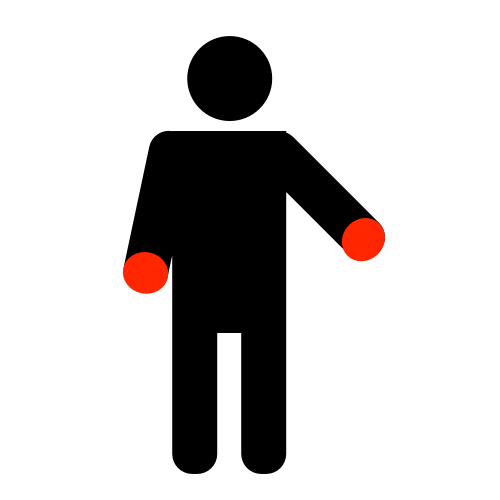
\includegraphics[height=120px]{figs/referee-signals/corner-kick-flipped.png}
        \caption{{\color{red}Corner Kick \textlangle{}red\textrangle{} Team} (on the half of the {\color{blue} blue} team)}
    \end{subfigure}
    \caption{\textbf{Corner Kick \textlangle{}color\textrangle{} Team.} One-handed signal. One arm, extended 45-degree \emph{down} in the direction of the team executing the corner kick. That is, right arm extended for the ``Blue team'' executing the corner kick on the ``Red team's'' side, and left arm extended for the ``Red team'' executing the corner kick on the ``Blue team's'' side. The non-signal hand is flat and motionless by the side of the body.}
\end{figure}
    
\begin{figure}[ht!]
    \centering
    \begin{subfigure}{.33\textwidth}
        \centering
        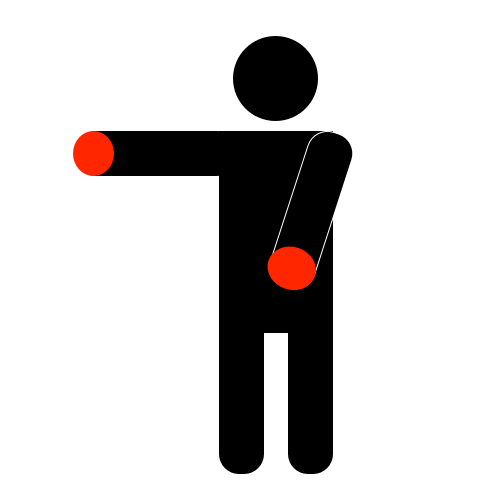
\includegraphics[height=120px]{figs/referee-signals/goal.png}
        \caption{\color{blue}Goal \textlangle{}blue\textrangle{} Team}
    \end{subfigure}
    \begin{subfigure}{.33\textwidth}
        \centering
        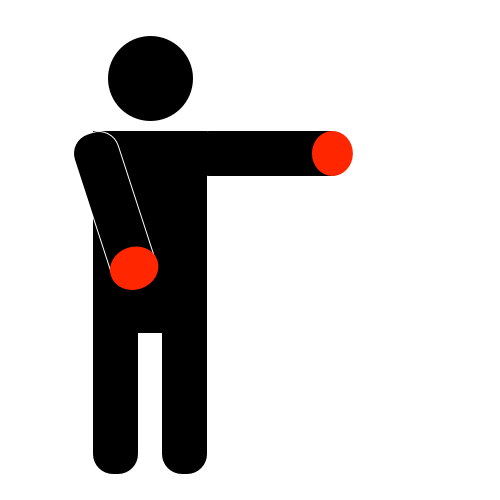
\includegraphics[height=120px]{figs/referee-signals/goal-flipped.png}
        \caption{\color{red}Goal \textlangle{}red\textrangle{} Team}
    \end{subfigure}
    \caption{\textbf{Goal \textlangle{}color\textrangle{} Team.} Two-handed signal. One arm, extended pointing at the center circle. Other arm, extended horizontally in the direction of the half of the field corresponding to the team that scored the goal. That is, right arm extended for the ``Blue team'', and left arm extended for the ``Red team''.}
\end{figure}

\begin{figure}[ht!]
    \centering
    \begin{subfigure}{.33\textwidth}
        \centering
        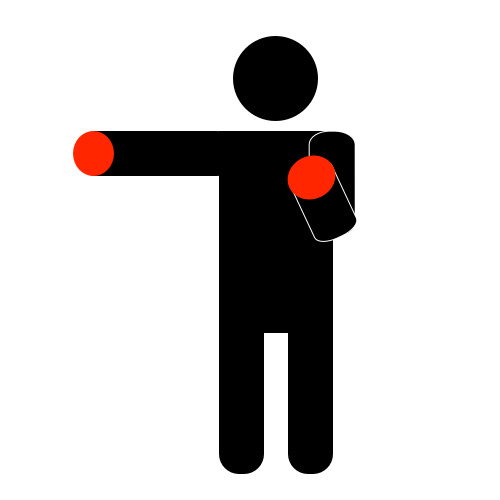
\includegraphics[height=120px]{figs/referee-signals/pushing.png}
        \caption{{\color{blue}Pushing Free-kick \textlangle{}blue\textrangle{} Team}\\ because a {\color{red}red} robot has pushed.}
    \end{subfigure}
    \begin{subfigure}{.33\textwidth}
        \centering
        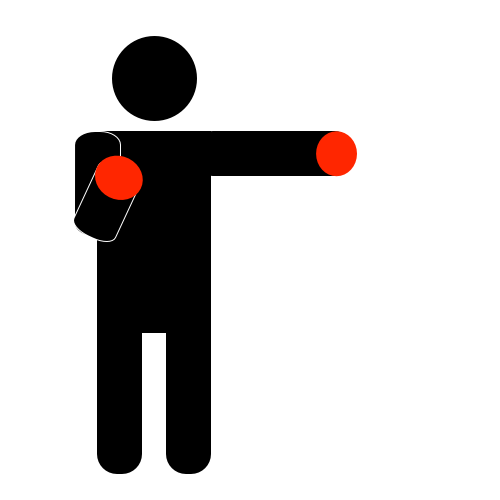
\includegraphics[height=120px]{figs/referee-signals/pushing-flipped.png}
        \caption{{\color{red}Pushing Free-kick \textlangle{}red\textrangle{} Team}\\ because a {\color{blue}blue} robot has pushed.}
    \end{subfigure}
    \caption{\textbf{Pushing Free-kick \textlangle{}color\textrangle{} Team.} Two-handed signal. One arm, vertical with bent elbow and palm facing in the direction of the extended arm. Other arm, extended horizontally in the direction of the half of the field corresponding to the team that is \emph{executing} the Free-kick. That is, left arm extended for the ``Red team'', and right arm extended for the ``Blue team''.}
\end{figure}

\begin{figure}[ht!]
    \centering
    \begin{subfigure}{.33\textwidth}
        \centering
        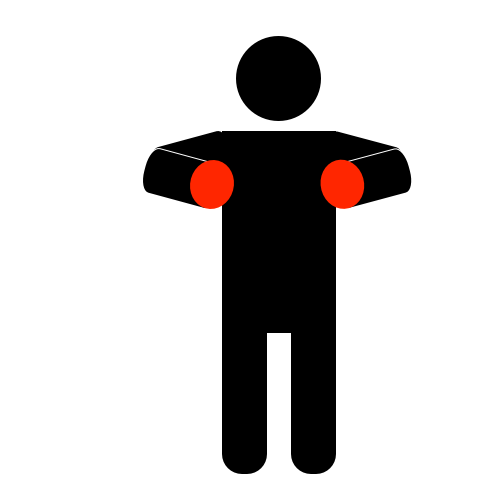
\includegraphics[height=120px]{figs/referee-signals/full-time-start.png}
        % \caption{Inner start point of the dynamic movement}
    \end{subfigure}
    \begin{subfigure}{.33\textwidth}
        \centering
        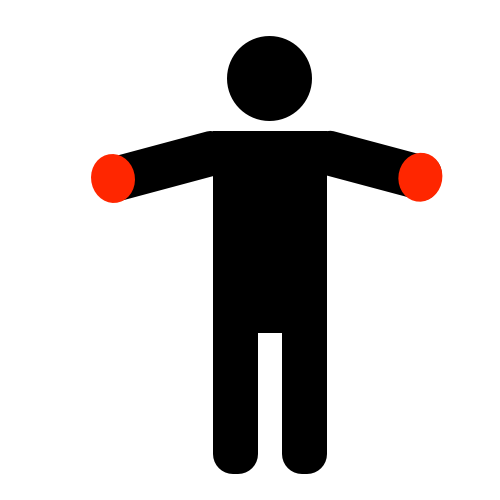
\includegraphics[height=120px]{figs/referee-signals/full-time-end.png}
        % \caption{Outer start point of the dynamic movement}
    \end{subfigure}
    \caption{\textbf{Full-Time.} Dynamic two-handed signal. Both arms slowly move symmetrically inward and outwards on a horizontal plane, bending at the elbows. Note, for the purpose of this challenge, the whistle associated with this signal should be a \textit{single} blow, unlike in normal SPL games.}
\end{figure}

\clearpage
\subsubsection{Challenge evaluation}
A team scores 1 point for every hand-signal that is correctly identified. A team scores an additional 1 point for correctly identifying the team corresponding to the signal (where appropriate: For a correct recognized \textit{Full-Time} signal without announcing a team, the team gets also 1 point for the team color). A team looses 1 point for incorrectly identifying a hand-signal (note a team may have a negative final score). The total time for the robot to identify each hand-signal is summed (If a robot fails to identify a hand-signal the time for the hand-signal is \qty{10}{\second}. If a robot incorrectly identifies a hand-signal, the time is how long the robot took to provide the incorrect identification).

Teams are ranked by their total points. In the event of tie-breaks, the team with the fastest total time to identify all hand-signals is ranked higher. The team with the highest total points, and lowest total time (for tie-breaks), wins the challenge.